\documentclass[]{article}
\usepackage{lmodern}
\usepackage{amssymb,amsmath}
\usepackage{ifxetex,ifluatex}
\usepackage{fixltx2e} % provides \textsubscript
\ifnum 0\ifxetex 1\fi\ifluatex 1\fi=0 % if pdftex
  \usepackage[T1]{fontenc}
  \usepackage[utf8]{inputenc}
\else % if luatex or xelatex
  \ifxetex
    \usepackage{mathspec}
  \else
    \usepackage{fontspec}
  \fi
  \defaultfontfeatures{Ligatures=TeX,Scale=MatchLowercase}
\fi
% use upquote if available, for straight quotes in verbatim environments
\IfFileExists{upquote.sty}{\usepackage{upquote}}{}
% use microtype if available
\IfFileExists{microtype.sty}{%
\usepackage{microtype}
\UseMicrotypeSet[protrusion]{basicmath} % disable protrusion for tt fonts
}{}
\usepackage[margin=1in]{geometry}
\usepackage{hyperref}
\hypersetup{unicode=true,
            pdftitle={Cards Analysis},
            pdfauthor={Eidan},
            pdfborder={0 0 0},
            breaklinks=true}
\urlstyle{same}  % don't use monospace font for urls
\usepackage{graphicx,grffile}
\makeatletter
\def\maxwidth{\ifdim\Gin@nat@width>\linewidth\linewidth\else\Gin@nat@width\fi}
\def\maxheight{\ifdim\Gin@nat@height>\textheight\textheight\else\Gin@nat@height\fi}
\makeatother
% Scale images if necessary, so that they will not overflow the page
% margins by default, and it is still possible to overwrite the defaults
% using explicit options in \includegraphics[width, height, ...]{}
\setkeys{Gin}{width=\maxwidth,height=\maxheight,keepaspectratio}
\IfFileExists{parskip.sty}{%
\usepackage{parskip}
}{% else
\setlength{\parindent}{0pt}
\setlength{\parskip}{6pt plus 2pt minus 1pt}
}
\setlength{\emergencystretch}{3em}  % prevent overfull lines
\providecommand{\tightlist}{%
  \setlength{\itemsep}{0pt}\setlength{\parskip}{0pt}}
\setcounter{secnumdepth}{0}
% Redefines (sub)paragraphs to behave more like sections
\ifx\paragraph\undefined\else
\let\oldparagraph\paragraph
\renewcommand{\paragraph}[1]{\oldparagraph{#1}\mbox{}}
\fi
\ifx\subparagraph\undefined\else
\let\oldsubparagraph\subparagraph
\renewcommand{\subparagraph}[1]{\oldsubparagraph{#1}\mbox{}}
\fi

%%% Use protect on footnotes to avoid problems with footnotes in titles
\let\rmarkdownfootnote\footnote%
\def\footnote{\protect\rmarkdownfootnote}

%%% Change title format to be more compact
\usepackage{titling}

% Create subtitle command for use in maketitle
\newcommand{\subtitle}[1]{
  \posttitle{
    \begin{center}\large#1\end{center}
    }
}

\setlength{\droptitle}{-2em}

  \title{Cards Analysis}
    \pretitle{\vspace{\droptitle}\centering\huge}
  \posttitle{\par}
    \author{Eidan}
    \preauthor{\centering\large\emph}
  \postauthor{\par}
      \predate{\centering\large\emph}
  \postdate{\par}
    \date{November 30, 2018}

\usepackage{booktabs}
\usepackage{longtable}
\usepackage{array}
\usepackage{multirow}
\usepackage[table]{xcolor}
\usepackage{wrapfig}
\usepackage{float}
\usepackage{colortbl}
\usepackage{pdflscape}
\usepackage{tabu}
\usepackage{threeparttable}
\usepackage{threeparttablex}
\usepackage[normalem]{ulem}
\usepackage{makecell}

\begin{document}
\maketitle

\subsection{Cards}\label{cards}

Hearthstone revolves around a set of roughly 1700 cards that can be
collected by players, put into decks, and then used in gameplay. Cards
are broadly divided into four types; in descending order of frequency:
Minions, Spells, Weapons, and Heroes. Cards may belong to one of nine
classes or be neutral and playable by any class.

\subsubsection{Minions}\label{minions}

Minions are characters that may be placed on the game board. Generally
they are used to threaten the opponent's hero or to defend against the
opponent's minions. The most basic attributes of a minion are its cost
to play, attack, and health. Minions may also have certain mechanics
that alter their behavior in-game.

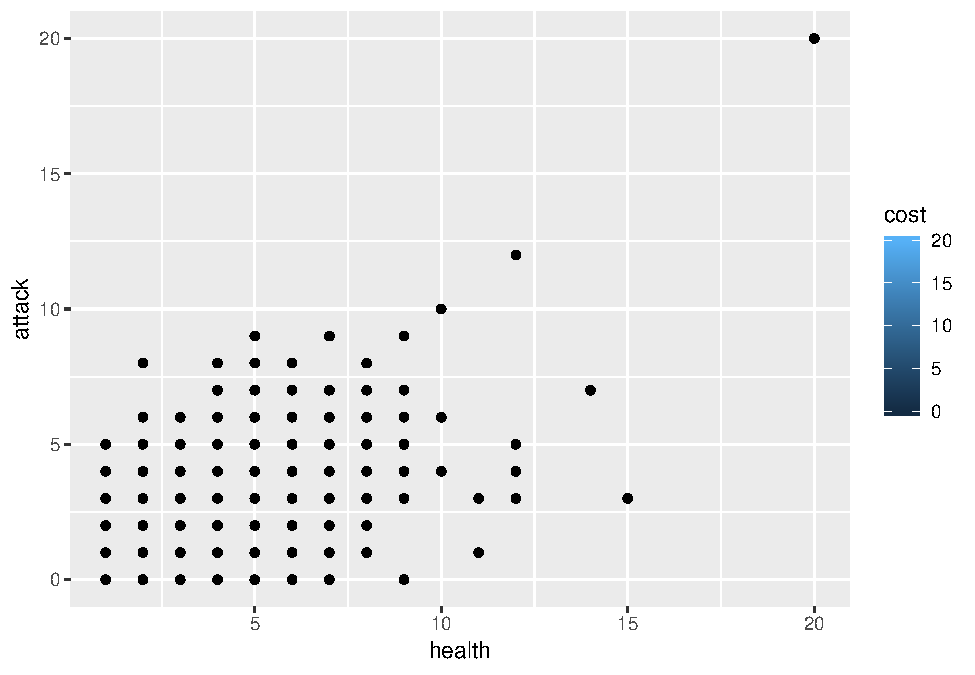
\includegraphics{cardsAnalysis_files/figure-latex/minions-plots-1.pdf}

\subsubsection{Spells}\label{spells}

\subsubsection{Weapons}\label{weapons}

\subsubsection{Heroes}\label{heroes}

\subsection{Appendix}\label{appendix}

I. Number of cards by type and class.

\begin{tabular}{l|l|r}
\hline
type & cardClass & n\\
\hline
MINION & NEUTRAL & 657\\
\hline
MINION & WARLOCK & 68\\
\hline
MINION & ROGUE & 63\\
\hline
SPELL & MAGE & 62\\
\hline
MINION & DRUID & 61\\
\hline
MINION & HUNTER & 61\\
\hline
SPELL & PRIEST & 59\\
\hline
MINION & PRIEST & 58\\
\hline
MINION & MAGE & 57\\
\hline
MINION & SHAMAN & 57\\
\hline
MINION & WARRIOR & 57\\
\hline
SPELL & DRUID & 56\\
\hline
SPELL & PALADIN & 54\\
\hline
MINION & PALADIN & 53\\
\hline
SPELL & HUNTER & 52\\
\hline
SPELL & SHAMAN & 51\\
\hline
SPELL & WARLOCK & 50\\
\hline
SPELL & ROGUE & 47\\
\hline
SPELL & WARRIOR & 44\\
\hline
WEAPON & WARRIOR & 16\\
\hline
WEAPON & PALADIN & 11\\
\hline
WEAPON & ROGUE & 9\\
\hline
WEAPON & SHAMAN & 9\\
\hline
WEAPON & HUNTER & 6\\
\hline
HERO & SHAMAN & 2\\
\hline
HERO & WARRIOR & 2\\
\hline
HERO & DRUID & 1\\
\hline
HERO & HUNTER & 1\\
\hline
HERO & MAGE & 1\\
\hline
HERO & PALADIN & 1\\
\hline
HERO & PRIEST & 1\\
\hline
HERO & ROGUE & 1\\
\hline
HERO & WARLOCK & 1\\
\hline
WEAPON & DRUID & 1\\
\hline
WEAPON & MAGE & 1\\
\hline
WEAPON & PRIEST & 1\\
\hline
WEAPON & WARLOCK & 1\\
\hline
\end{tabular}


\end{document}
